\documentclass[11pt,a4paper]{report}

\usepackage[margin=1.0in]{geometry}
\usepackage{polytechnique,url}
\usepackage{graphicx}
\usepackage{pdfpages}

\title{Specifications for the Attitude Control and Determination System-XCubeSat} 
\author{Dhruv Sharma, Damien Seux, Quentin Lisack, Kevin Garanger}

\date{12 April 2015} 

\renewcommand{\titrecourt}{Specifications ADCS}
\setcounter{secnumdepth}{5}
\begin{document}
\maketitle

\tableofcontents
\listoffigures

\chapter{Introduction}

The objective of this document is to summarize in one place the specifications related to the software of the Attitude Control and Determination System, henceforth ADCS of the nano-satellite X-CubeSat developed by the students of École Polytechnique, Paris. We have divided the document into the following sections 

\begin{itemize}
\item 
Definition of the architecture of the ADCS 
\item 
External Interfaces available on the ADCS 
\item 
Sensors and peripherals on the ADCS 
\item 
Data formats used for computing 
\item 
Protocols for testing 
\end{itemize}

This document shall be useful for all people currently concerned with the conception of the ADCS and eventually for students who will take over the project in the months to come. This document is however, far from being complete and additions, corrections and deletions will be made till the day of delivery. 

\chapter{Architecture of the ADCS}\thispagestyle{fancy}

The ADCS uses a microprocessor manufactured by ST Microelectronics based on the ARM Cortex-M4 Architecture. The model used is STM 32F405 RGT6

The available interfaces, sensors and other peripherals available on the ADCS are: 

\begin{itemize}
\item 
32 MB External Memory  
\item 
7(or 9) sun sensors 
\item 
Magnetometer
\item 
Gyrometer
\item 
H-Bridges to modulate power to the magneto-torquers 
\item 
A Serial interface with the On-Board Computer (\textit{Ordinateur de Bord} henceforth, ODB) 
\end{itemize}

Following is the complete plan for the ADCS: 

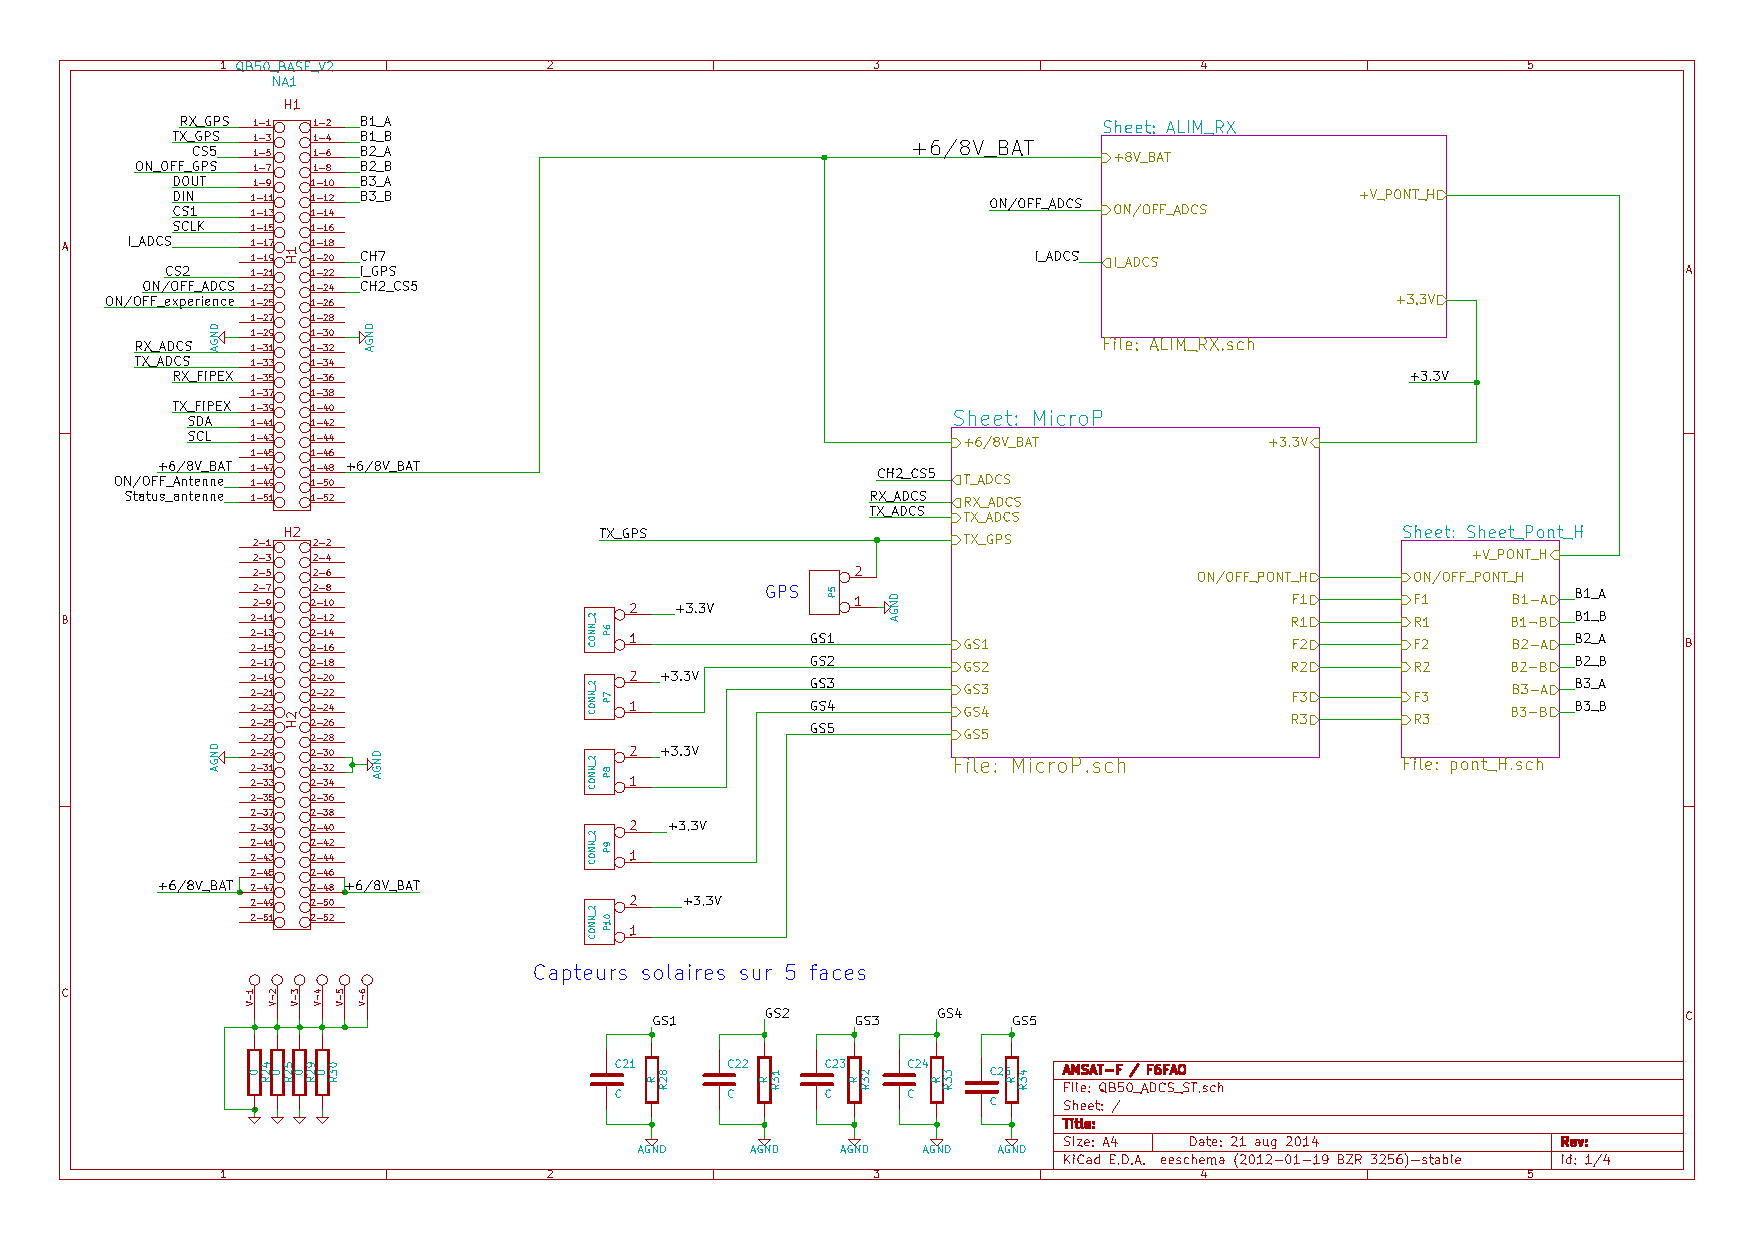
\includepdf[pages={-},angle=90]{QB50_ADCS_ST.pdf}

\chapter{External interfaces} \thispagestyle{fancy}



\chapter{Software Architecture} \thispagestyle{fancy}

\section{Division of the software} 
 
The ADCS software is divided into the following layers 

\begin{enumerate}
\item 
\textbf{API Firmware}: In this layer, all the low-level functionalities are collected. By low-level functionalities, we mean all those functionalities which are not directly relevant to the functioning of the algorithms. This layer doesn't provide any data to the algorithms. Rather, this layer is concerned only with initializing and configuring the various peripherals that we have on the ADCS.
\item 
\textbf{Driver}: jhis layer acts as a bridge between the lower level API firmware and the higher-level specialized functions that we require to run our algorithms. Ideally, in this layer we find the functions which get the raw data from the sensors, convert or calibrate them as necessary and send them to the algorithms for further use.
\item 
\textbf{Specialized Functions}: The specialized functions are the functions which implement the algorithms for determining and controlling the attitude of the satellite. These functions are high-level functions and require the data provided to them by the \textit{Driver} layer above to function. 
\end{enumerate}

\begin{figure}[!h]
\centering 
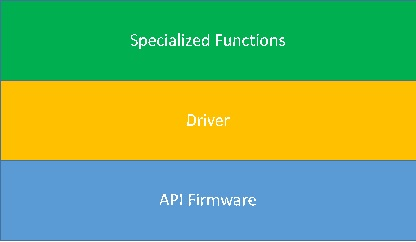
\includegraphics[width=10cm]{arch_layers.jpg}
\caption{\textit{Division of the software in three layers each independent of the other}}
\label{layers_arch_soft}
\end{figure}


\section{Structure of classes} 
Once we have abstracted the software as being divided into layers depending on the kind of functions we will write for the software, we consider next the division of the software into dedicated classes. The class structure as envisaged for the ADCS is summarized in the graph below. The arrow head signifies that the a particular class gets a particular piece of data from the class where the arrow originates. 

\begin{figure}[h]
\centering 
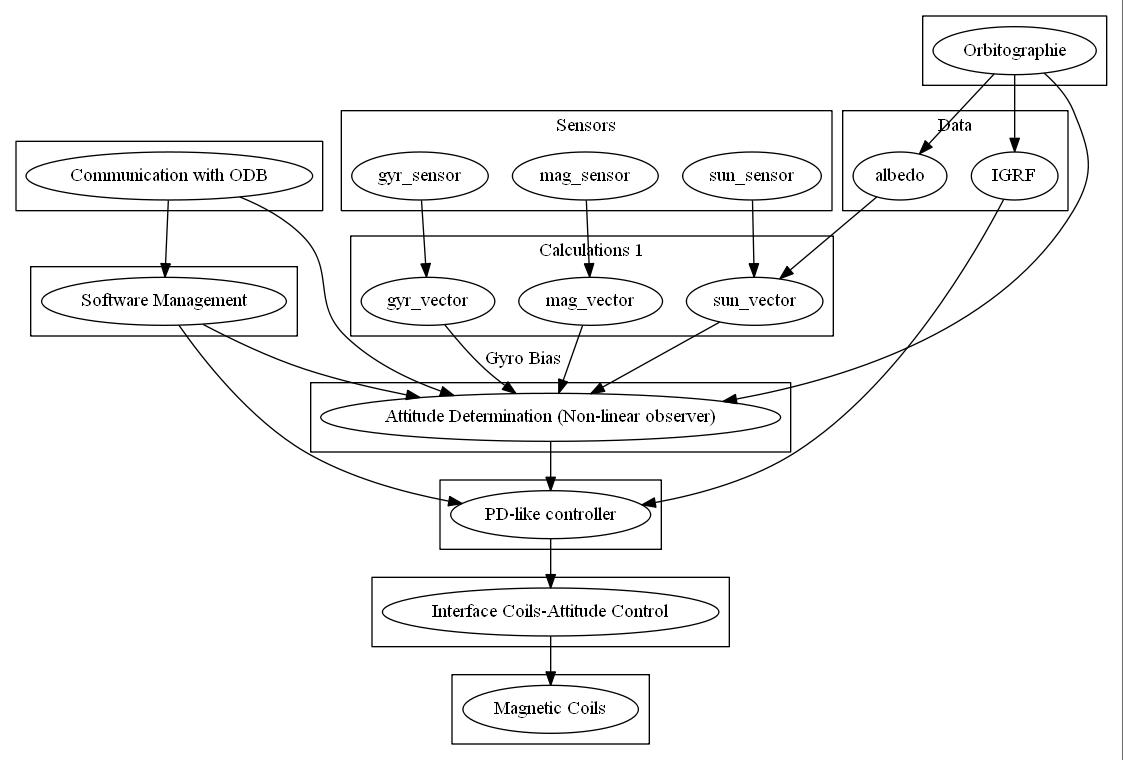
\includegraphics[scale=0.6]{class_structure}
\caption{\textit{Class structure for ADCS Software}}
\label{struct_class}
\end{figure}


\begin{enumerate}
\item 
\textbf{Calculations 1}: This layer consists of a first layer of calculations effectuated once raw data is received from the sensors. In this layer, we receive the raw data from the sun-sensors, magnetometer and the gyrometer. 

\item 
\textbf{Calculations 2}: This corresponds to a supplementary layer of calculations which is effectuated once the raw data has been received. This step might take different forms for different sensors. For instance, once we have received the sun sensor raw data, the supplementary steps include converting the raw data into a voltage and further combining the data from the 9 sun-sensors into one sun-vector with three components. For the magnetometer however, we can eventually consider calibrating the data with the temperature. Identically for the gyrometer as well. 

This layer also corresponds to the calculations to be done to configure the magneto-torquers. The magneto-torquers are controlled by Pulse-Width Modulation(PWM). For PWM, we require the frequency of modulation (in KHz) and the duty cycle (in percent). The result of the algorithms, however, is the magnetic moment to be generated by the magnetic torquers. Thus we require precise data on the behaviour of the magnetic coils used to convert this magnetic moment into a duty-cycle. (The frequency of modulation shall be fixed for all the coils)

Finally, this step also relates to reading the terrestrial magnetic field map and the albedo map from the external memory. All this data once collected, calibrated and treated will be given to the algorithms, which we explain below. 

\item 
\textbf{Attitude Determination and Control Phase}: Once the data has been generated (after eventual calibrations), we have the layer where the actual control of the satellite takes place. The details of the algorithms will be presented in an ulterior section. 

The output of the algorithms is the magnetic moment to be generated in each of the magnetic coils. 
\end{enumerate}


As mentioned earlier, the ADCS disposes the following list of peripherals: 


\begin{itemize}
\item 
32 MB External Memory  
\item 
7(or 9) sun sensors 
\item 
Magnetometer
\item 
Gyrometer
\item 
H-Bridges to modulate power to the magneto-torquers 
\item 
A Serial interface with the On-Board Computer (\textit{Ordinateur de Bord} henceforth, ODB) 
\end{itemize}

Each of these peripherals need to be configured and their outputs need to be specified so that the algorithms used for the determining and controlling the attitude function optimally. 



\chapter{Data formats}\thispagestyle{fancy}

\chapter{Testing}\thispagestyle{fancy} 


\end{document}